% % Double-spaced
%\usepackage{setspace}
%\onehalfspacing

\section*{Abstract}

\subsection*{Background}

Children with oropharyngeal dysphagia have impaired airway protection mechanisms and are at higher risk for pneumonia and other pulmonary complications.
Aspiration of gastric contents is often implicated as a cause for these pulmonary complications, despite being supported by little evidence.
The goal of this study is to determine the relative contribution of oropharyngeal and gastric microbial communities to perturbations in the lung microbiome of children with and without oropharyngeal dysphagia and aspiration.

\subsection*{Methods}

We conducted a prospective cohort study of 222 patients consecutively recruited from a tertiary aerodigestive center undergoing simultaneous esophagogastroduodenoscopy and flexible bronchoscopy.
Bronchoalveolar lavage, gastric and oropharyngeal samples were collected and 16S sequencing was performed.
A subset of patients also underwent video fluoroscopic swallow studies to assess swallow function and were categorized as aspiration/no aspiration.
Microbial communities across the aerodigestive tract were compared in patients with and without aspiration by calculating within-patient beta diversities and quantifying microbial exchange across sites.

\subsection*{Results}

Within all patients, lung, oropharyngeal and gastric microbiomes overlap.
The degree of similarity is the lowest between the oropharynx and lungs (median Jensen-Shannon distance (JSD) $=$ 0.90), and as high between the stomach and lungs as between the oropharynx and stomach (median JSD $=$ 0.55 and 0.56, respectively; p $=$ 0.6).
Unlike the oropharyngeal microbiome, lung and gastric communities are highly variable across people and driven primarily by person rather than body site.
In patients with aspiration, the lung microbiome more closely resembles oropharyngeal rather than gastric communities and there is greater prevalence of microbial exchange between the lung and oropharynx than between gastric and lung sites (p $=$ 0.04 and 3x10$^{-5}$, respectively).

\subsection*{Conclusions}

The gastric and lung microbiomes display significant overlap in patients with intact airway protective mechanisms while the lung and oropharynx remain distinct.
In patients with impaired swallow function and aspiration, the lung microbiome shifts towards oropharyngeal rather than gastric communities.
This finding may explain why antireflux surgeries fail to show benefit in pediatric pulmonary outcomes.

\newpage
\section{Introduction}

The economic and social impact of oropharyngeal dysfunction and aspiration is well known in the adult stroke population; adults with oropharyngeal dysfunction are at greater risk of pneumonia than those without \cite{holas1994aspcomplications}.
Little is known about aspiration-related lung disease in children, though recent studies suggest that up to 10\% of all pneumonia hospitalizations in pediatrics are related to aspiration \cite{thomson2016asppneumo}.
Clinicians often assume these pneumonias result from the aspiration of refluxed gastric contents and frequently treat these children with antireflux surgery, fundoplication.
Despite this common surgical practice, there are no pediatric studies which conclusively show improved pulmonary outcomes after fundoplication, suggesting that the respiratory symptoms seen in aspirating patients may not be related to aspiration of gastric contents \cite{barnhart2013fundo,lee2008fundo,goldin2006fundo,yeh2016,srivastava2009fundo}.
An alternative hypothesis is that aspiration-related respiratory symptoms may result from aspirated oropharyngeal contents.
To test this hypothesis, we determined the microbial signatures of the lungs, stomach, and oropharynx in children with and without oropharyngeal dysphagia (i.e. with and without impaired airway protective mechanisms) to determine the relative contributions of the oropharyngeal and gastric microbiomes to the lung microbiome.

Previous studies have shown that the mouth, upper respiratory tract, and lung microbiota contain similar microbes, and that upstream oral communities seed downstream sites (e.g. lungs and stomach) \cite{Bassis2015source,Charlson2011topographical,rosen2015ppi}.
However, there is little consensus on whether there exists a distinct or "core" lung microbiome that is consistent across people \cite{Charlson2011topographical,venkataraman-2015-dispersal,segal-2013-pneumotypes,erbDownward-2011-COPD}.
Most studies, however, agree that the lung microbial communities share taxa with the oral microbiome, but that there are some bacteria present in lung communities whose abundances cannot be traced solely to the mouth \cite{Bassis2015source,Charlson2011topographical,morris-2013-healthsmokers,segal-2013-pneumotypes}.

While the importance of oropharyngeal flora in seeding the lungs has been heavily studied in ICU settings \cite{tantipong2008decontamination,koeman2006decontamination,hu2010pseudo}, the role of oropharyngeal-lung flora exchange in otherwise heathy children with isolated swallowing dysfunction is unknown.
Furthermore, studies investigating the relationships between microbial communities across the aerodigestive tract have not examined how microbes exchange between the stomach and lungs, and how this exchange relates to clinical factors such as aspiration and gastroesophageal reflux.

If the lung microbiome of aspirating patients exhibits more exchange with the oropharynx than the stomach, this could provide evidence for why anti-reflux surgery is not helpful in patients with aspiration-related respiratory symptoms.
Furthermore, a shift in the lung microbial communities toward an oropharyngeal population could not only result in overt pneumonia but may also have more subtle, pro-inflammatory effects \cite{segal-2016-inflammation}.
Finally, if there is a unique aerodigestive microbial signature in aspirating patients, microbial profiling may be helpful as a diagnostic tool for oropharyngeal dysphagia.

\section{Methods}

\subsection{Patient cohort and sample collection}

We conducted a prospective cross sectional cohort study of children ages 1--18 undergoing bronchoscopy and esophagogastroduodenoscopy (EGD) for the evaluation of chronic cough.
Patients with gastrostomy or nasogastric tubes, a history of gastrointestinal surgery, or antibiotics within 4 weeks of sample acquisition were excluded.
The study was approved by the Boston Children's Hospital Institutional Review Board and informed consent was obtained from all patients/parents.

We first performed brushing of the posterior tongue to obtain oropharyngeal samples, placing the brush in TE buffer at -80C.
Second, the bronchoscopy and bronchoalveolar lavage (BAL) was performed through an endotracheal tube in distal airways of the right middle lung or the most visually inflamed lung.
Finally, gastric sampling was performed during the EGD.
The endoscope was advanced, without suctioning, immediately into the stomach where the gastric fluid was suctioned into a sterile leukitrap.
A minimum of 1 cc of gastric and lung fluid were collected and transferred to -80C.
Each patient had a triad of samples collected: oropharynx, gastric fluid, and BAL (Tables \ref{tab1} and \ref{tab2}) \cite{rosen2015ppi}.

\subsection{Multichannel intraluminal impedance with pH (pH-MII)}

A subset of patients had pH-MII testing at the discretion of the patient's primary gastroenterologist.
Acid reflux episodes were defined as episodes detected by the impedance (MII) sensors with associated drop in pH to $<$ 4; non-acid episodes did not have the associated drop.
The percentage of time that reflux was in the proximal/distal esophagus was calculated by dividing the sum of the bolus clearance times in the proximal/distal esophagus by the total study duration.
The percentage of full column reflux events was defined as the percentage of the total reflux events that reached the proximal two impedance sensors (i.e., the proximal most impedance channel) \cite{rosen2004impedance}.

\subsection{Oropharyngeal dysphagia assessment}

A subset of the patients included in this study had a videofluoroscopic swallow study (VFSS) to asses swallow function and were divided into two groups (normal swallow function and aspiration/penetration).
Because patients with penetration on VFSS have similar pulmonary symptoms and respond similarly to thickening as patients that aspirate, we included patients with aspiration and penetration in one group.

\subsection{Sample processing and sequencing}

Oropharyngeal swabs, BAL, and gastric fluid samples suspended in Tris-Saline buffer were centrifuged for 3 minutes at 10,000 rcf prior to DNA isolation.
DNA was extracted from the sample pellet with the Qiagen DNeasy PowerSoil Kit as described by the manufacturer, with the following modifications: protein precipitation in one step using 100 $\mu$L of each C2 and C3 solutions, and column centrifugation at 10,000 rcf for 10 minutes.
Sequencing was performed in two batches at the Broad Institute.
Patients with multiple samples had all of their respective samples sequenced in the same batch.

\subsection{Microbiome data processing and analysis}

Paired end reads were merged using USEARCH \texttt{-fastq\_mergepairs} and truncated to 200 bp.
Reads with more than 2 expected errors were discarded.
Operational taxonomic units (OTUs) were clustered at 99\% similarity and assigned taxonomy using the RDP classifier (c $=$ 0.5) \cite{wang2007rdp}.
All quality filtering and OTU calling steps were performed with an in-house pipeline \\ (https://github.com/thomasgurry/amplicon\_sequencing\_pipeline).

Beta diversity was calculated with the Jensen-Shannon distance (JSD).
Only samples which were sequenced in the same batch were considered in cross-patient comparisons.
Differences in overall community structure across sites was assessed using the PERMANOVA test as implemented in scikit-bio v 0.4.2 (\texttt{skbio.stats.distance.permanova}).

To define exchanged OTUs, we used data from patients with all three sites sequenced.
For each OTU, we calculated the Spearman partial correlation ($\frac{r_{xy} - r_{xz}r_{zy})}{\sqrt{(1 - r_{xz}^2)(1 - r_{zy}^2)}}$) between its non-zero abundances in two sites, partialled on the third site (Scipy v 0.19.0 \texttt{stats.spearmanr}).
P-values for each OTU were calculated as the percentage of null correlations larger than the observed correlation after shuffling abundances 2000 times.
Only OTUs present in two sites in at least 10 patients were considered.
OTUs with FDR-corrected q-value $<$ 0.1 were defined as ``exchanged'' (\texttt{sandbox.stats.multicomp.multipletests} with \texttt{method=`fdr\_bh'}).
To determine the statistical significance of the number of exchanged OTUs, we shuffled the patient IDs for each OTU in each site and re-defined ``null'' exchanged OTUs as described above.

We used five-fold cross-validation and Random Forest classifiers (scikit-learn v 0.18.1 \newline \texttt{ensemble.RandomForestClassifier} with n\_estimators=1000) for all supervised machine learning analyses.
Areas under the ROC curve (AUCs) were calculated based on the predictions on each fold's test set (mean values across folds is reported) and Fisher p-values were calculated from all test set predictions.
The aspiration/non-aspiration classifiers varied different train/test splits, so we report the mean results across 100 repetitions.

\subsection{Availability of data and materials}
Code to reproduce the analyses presented here are available at www.github.com/cduvallet/aspiration-analysis-public.
The 16S sequencing data used in this study will be made available in the SRA repository at accession number SRP141148 upon publication and clinical metadata are available upon request from the corresponding author.

\section{Results}

Two hundred and twenty two patients were included in the analysis (Tables \ref{tab1} and \ref{tab2}).
The mean age of the patients was 7.1 $\pm$ 5.4 years.
One hundred out of 222 patients were taking proton pump inhibitors at the time of sampling.
One hundred and four patients had a videoflouroscopic swallow study of which 47 (45\%) had evidence of aspiration or penetration and 57 (55\%) had normal swallow function.
Thirty one patients had pH-MII testing for gastroesophageal reflux at the time of sample collection.

\subsection{Aerodigestive microbiome across people}

%To \textbf{characterize the baseline composition of aerodigestive communities}, we examined patients who had all three sites (oropharyngeal swab, lung, and gastric fluid) sequenced (Table \ref{tab:intra_samples}).
%Similarly to the adult aerodigestive microbiome,
At the genus level, pediatric aerodigestive communities share many predominant members, including \textit{Streptococcus}, \textit{Prevotella}, \textit{Haemophilus}, \textit{Veillonella}, and \textit{Neisseria} (Figure \ref{fig1}).
Despite genus-level similarities, OTU-level aerodigestive communities are distinct and highly variable across people.
The overall community composition was significantly different between sites (PERMANOVA on JSD, p $<$ 0.001, Figure \ref{fig2}B).
Furthermore, lung communities were very different across people (median lung-lung JSD $=$ 0.88) while oropharyngeal communities tended to be more similar (median oropharyngeal-oropharyngeal JSD $=$ 0.59, Figure \ref{fig2}A).

%These findings point to a lack of an OTU-level ``core'' lung microbiome, and complicate the search for reliable non-pathogenic microbial biomarkers in the lung microbiome, since most patients will have few lung OTUs in common with other patients.

%Proteobacteria and Firmicutes were the most abundant phyla in the aerodigestive microbiome, comprising more than half of the relative abundance in all three sites.
%\textit{Streptococcus} and \textit{Haemophilus} were among the top three most abundant genera in all three sites.
%\textit{Prevotella} was the most abundant genus (21\% average abundance) in the oropharyngeal samples and among the top ten most abundant genera in the other sites (9\% and 3\% average abundance in gastric fluid and lungs, respectively).

%\textbf{Despite similar genus-level taxonomic profiles, aerodigestive sites are distinct and variable across people.}


\subsection{Aerodigestive microbiome within people}

We compared aerodigestive communities within patients who had multiple sites sequenced (Table \ref{tab2}, Figure \ref{fig3}).
Oropharyngeal and gastric fluid communities are similar within patients (median JSD $=$ 0.56), reflecting that the mouth seeds the gastric microbiome \cite{Bassis2015source,Charlson2011topographical}.
The majority of patients had very different lung and oropharyngeal communities (median JSD $=$ 0.90), and these differences were significantly higher than either the lung-gastric fluid or gastric fluid-oropharyngeal beta diversities (p $< 1 \times 10^{-8}$, Figure \ref{fig3}A).
Surprisingly, lung and stomach communities were as similar to each other as stomach and oropharyngeal communities (median JSD $=$ 0.55 versus median JSD $=$ 0.56, respectively, p $=$ 0.6).
%One possible explanation for these similar gastric and lung communities is that they are both being seeded by the oropharynx, resulting in similar compositional profiles \cite{Bassis2015source,venkataraman-2015-dispersal}.
%Alternatively, as our data has previously suggested, the lungs and stomach may directly exchange bacteria through microaspiration of gastric contents or coughing and subsequent swallowing \cite{rosen2011culture}.
%Finally, both the lungs and stomach have low biomass and harsh selective pressures, which may lead to similar community taxonomic profiles without necessarily requiring direct exchange of individual bacteria \cite{Bassis2015source,venkataraman-2015-dispersal,Dickson2014}.

To identify specific microbes exchanging between sites, we reasoned that an actively exchanging microbe's abundances in two sites should be correlated across patients (Supplementary Figure A-1 and Methods).
We identified 12 OTUs exchanged between lung and oropharyngeal, 74 between gastric fluid and lung, and 118 between oropharyngeal and gastric fluid communities.
These results were statistically significant: we found a maximum of 2 exchanged OTUs between sites in our null analysis.
The low number of directly exchanged OTUs between the oropharynx and lungs supports the finding that these sites are more distinct than others in the aerodigestive tract.
The lungs and stomach exchange fewer OTUs than the oropharynx and stomach even though they have comparable intra-patient similarities, suggesting that factors other than specific bacterial exchange contributes to the similarity between lungs and stomachs within patients.

Random Forest classifiers trained to distinguish between sites (ensuring that samples from the same patient were in the same train/test set) were able to identify a generalizable oropharyngeal microbial signature that distinguishes the oropharynx from other sites across people (AUC $=$ 0.95 for both gastric fluid and lung comparisons, Figure \ref{fig3}B).
Surprisingly, when we compared within-patient similarities across sites to across-patient similarites for the same sites, we found that lung and stomach communities within patients were more similar than lungs across patients and than stomachs across patients (Table \ref{tab3}, p $< 1 \times 10^{-8}$).
Thus, while there exists a ``core'' oropharyngeal microbiome across people, lung and gastric communities are more variable and driven primarily by the person rather than body site.
These results challenge the prevailing hypothesis that human-associated microbial communities are primarily driven by body habitat and instead suggest that patient-specific relationships may be equally, if not more, important in determining community structure in the aerodigestive microbiome \cite{costello2009bodysites,huttenhower2012hmp,lozupone2013bodysites}.

\FloatBarrier

\subsection{Aspiration modulates the relationship between lung and oropharyngeal microbiomes but not the lung and stomach}

Next, we investigated the impact of oropharyngeal dysphagia and aspiration on the relationships between aerodigestive microbiomes.
Aspirators had significantly more similar lung and oropharyngeal communities than non-aspirators (Figure \ref{fig4}A, p $=$ 0.04) and were much more likely to have the pre-defined oropharyngeal-lung microbes in both their oropharynx and lungs than non-aspirators (p $= 2 \times 10^{-5}$) (Figure \ref{fig4}B).
Lung-oropharynx exchanged OTUs co-occurred in a median of 42\% of aspirators' lung and oropharyngeal communities but only 20\% of non-aspirators'.
Aspirators were not more likely to have stomach-lung microbes present in both the lungs and gastric fluid than non-aspirators (Figure \ref{fig4}B, p $>$ 0.5), and lung and gastric communities of aspirating patients were not necessarily more similar to each other than those of non-aspirating patients (Figure \ref{fig4}A, p $=$ 0.5).

To identify potential microbial biomarkers of aspiration, we looked at the exchanged OTUs which were most frequently present in the lung and oropharyngeal communities of aspirators relative to non-aspirators.
In the oropharyngeal-lung exchanged OTUs, these were an unknown OTU in the \textit{Flavobacteriaceae} family, OTUs in the \textit{Fusobacterium}, \textit{Rothia}, \textit{Veillonella} genera, and an unknown OTU in the \textit{Prevotellaceae} family, among others (Table \ref{tab4}, gastric-lung OTUs in Supplementary Table A-1).

We used Random Forest classifiers trained on the presence of exchanged OTUs in different sites to test their potential as biomarkers.
The concordant presence or absence of exchanged OTUs in the two sites improved classifiers based on the oropharyngeal-lung OTUs but not the ones based on the lung-gastric OTUs, relative to classifiers based on the presence of the exchanged OTUs in either site alone (Table \ref{tab5}).
Using Random Forest classifiers trained on the entire microbiomes, we found that combining the oropharynx and lung communities resulted in a better classifier than either community alone (Table \ref{tab6}).
Surprisingly, the classifiers trained on oropharyngeal and gastric communities performed well, despite our expectation that aspiration-induced changes in the microbiome would manifest in the lungs rather than the oropharynx or stomach.
We confirmed that the patients' aspiration status was not confounded with proton pump inhibitor usage (Fisher exact p-value $>$ 0.2), but there may be other co-morbidities or unmeasured confounders that could be driving the differences detected in these communities.
However, taken together, these results suggest that identifying a biomarker for aspiration based on bacteria in both the lungs and oropharynx may be possible, and that these two sites together contain more information about a patient's aspiration status than either site alone.

\FloatBarrier

\subsection{Reflux may impact the relationship between lung and stomach microbiomes}

Reflux profiles for the 31 patients are shown in Table \ref{tab7}.
The percent of full column, distal, and proximal reflux were slightly negatively correlated with gastric-lung JSD, indicating that patients with more frequent reflux may have more similar gastric and lung microbial communities (Figure \ref{fig5}).
However, the large range of gastric-lung JSDs across all patients and relatively weak correlation suggests that other non-reflux factors likely contribute more to the similarities between gastric and lung communities that are observed across all people.

%Due to insufficient patients with both pH-MII and VFSS testing, we were unable to determine whether the relationship between reflux and lung-gastric similarity was more pronounced in patients with impaired airway protective mechanisms.
%However, our previous results that aspiration from the oropharynx has a larger effect on lung microbial communities than aspiration from the stomach suggest that this is likely not the case.
%Thus, if reflux is not a primary driver of microbial exchange between the stomach and lungs, efforts to reduce microbial exchange should not focus exclusively on reflux-related factors but should also consider preventing aspiration from the mouth.

\FloatBarrier

\section{Discussion}

In this study, we characterized the relationships between the oropharyngeal, lung, and gastric microbiomes in a large pediatric cohort with and without swallowing dysfunction.
Leveraging our simultaneous sampling of multiple sites per patient, we find that there exists a ``core'' oropharyngeal microbiome across patients, that the lung and gastric communities are highly variable across patients and driven primarily by patient rather than body site, and that within patients the lung and oropharyngeal communities remain most distinct.
We show for the first time that in patients with impaired swallowing, the lung microbiome shifts toward oropharyngeal flora rather than gastric flora.
Our results also suggest that identifying biomarkers for aspiration based on the presence of certain bacteria in both the lungs and oropharynx may ultimately be possible.
% We also show that, despite the common perception that gastroesophageal reflux results in microbial changes in the lung, gastroesophageal reflux did not have a large effect on the relationship between lung and gastric microbial communities, suggesting that other mechanisms contribute more to microbial exchange between these sites

There are several limitations to our study.
First, because it is unethical to perform bronchoscopies on healthy children, our patients in this study had respiratory symptoms.
However, we believe that our patient population represents patients typically seen in aerodigestive centers and that understanding the degree of microbial exchange is most clinically relevant in patients with symptoms.
The microbial populations we found in this study are similar to those of previously published studies of both healthy and symptomatic adults which reinforces the validity of our results \cite{Bassis2015source,Charlson2011topographical,erbDownward-2011-COPD,morris-2013-healthsmokers}.
Second, the number of patients undergoing pH-MII testing was relatively small which limits our conclusions about the impact of gastroesophageal reflux on the lung.
However, our study raises enough concerns about the significance of oropharyngeal-lung exchange in children with impaired swallowing that gastroesophageal reflux should not be considered as the primary source of microbial exchange causing pulmonary symptoms.
Third, the diagnosis of oropharyngeal dysphagia in this study was based on VFSS.
While this only categorizes patients based on a ``one-point-in-time'' study, it is the gold standard test to diagnose oropharyngeal dysphagia in children and therefore we feel it is appropriate for use in this study.

Despite these limitations, our findings have broad clinical implications for the understanding and treatment of oropharyngeal dysphagia with resultant aspiration.
Our clinical finding that the lung microbiome in children with aspiration shifts toward the oropharynx rather than the stomach highlights the importance of understanding the primary driver of microbial exchange so that therapies can be tailored accordingly.
For example, if the mechanism of lung symptoms and disease in aspirating children results from a microbial shift towards oropharyngeal flora, anti-reflux surgery will be of no benefit to preventing oropharyngeal-lung exchange.
Instead, therapies may need to be tailored to focused on changing oropharyngeal flora or salivary properties.

While there are no existing pediatric microbiome studies of the aerodigestive microbiome in patients with dysphagia, there is evidence that children with oropharyngeal dysphagia are predisposed to pneumonia and that this could be due to increased aspiration of microbes from the oral microbiome.
In a study of 382 children undergoing VFSS, evidence of aspiration predicted pneumonia risk, though the causative organisms for these pneumonias were not known \cite{weir2007pneumoasp}.
In cohort of elderly aspirating patients, oral colonization by respiratory pathogens was associated with increased risk of pneumonia, highlighting the potential importance of oral flora in influencing the lung outcomes \cite{ortega2015oralpatho}.
Finally, a previous study of healthy adults found that individuals with oropharyngeal bacteria in their lungs had increased evidence of inflammatory metabolomic signals, suggesting that even a change of lung flora to commensal oropharyngeal bacteria can trigger inflammation even in healthy patients \cite{segal-2016-inflammation}.
Our results add to these findings and suggest that changes in the lung microbiome towards oropharyngeal flora merit additional study to determine if these shifts result in increased morbidity or worse clinical outcomes, including the development of pneumonia.

From a microbial perspective, we identified bacterial families and genera that are more commonly exchanged between the oropharynx and lungs of children that aspirate than of children with intact swallowing mechanism.
While there are no other 16S sequencing studies determining aspiration pneumonia risk in children, there is evidence from the adult literature that similar bacteria are involved in aspiration pneumonia risk.
For example, oropharyngeal \textit{Streptococci} were found to be more abundant in the lungs of adults with pneumonia and aspiration risk factors than without aspiration risk \cite{akata2016oralstrepto}.
In a study of 173 adults in long term care facilities, patients with oropharyngeal \textit{Prevotella} and \textit{Veillonella} had increased risk of death from pneumonia compared to patients who had oropharyngeal \textit{Neisseria} and \textit{Fusobacterium} \cite{kageyama2017pneumomortality}.
Our study is a critical first step toward identifying bacteria present in the oropharynx and lungs of aspirating children that may result in higher risk for pneumonias, with additional studies needed to determine their impact on pediatric outcomes.

In summary, our findings suggest that interventions to reduce aspiration-related respiratory complications due to increased microbial exchange should target aspiration from the oropharynx rather than the stomach.
This microbial data supports the clinical observation that antireflux surgery fails to prevents pulmonary complications such as pneumonias or hospitalizations \cite{barnhart2013fundo,lee2008fundo,goldin2006fundo,yeh2016,srivastava2009fundo}.
By simultaneously sampling multiple sites per patient, we show that the lung and stomach microbiomes are highly variable across patients and determined primarily by patient rather than body site.
Understanding the relationships between aerodigestive communities in aspirating and non-aspirating patients provides insight into the potential pathophysiology behind aspiration-related respiratory outcomes and suggests potential diagnostics and therapeutics for future investigation.

\section{Declarations}

\subsection{Acknowledgments}

We thank Scott Olesen and Manu Kumar for helpful discussions on statistical analyses, and Nathaniel Chu and members of the Alm lab for helpful discussions on presenting and visualizing the results.

\subsection{Funding}

This work was supported by NIH R01 DK097112 (R.R.), the Boston Children's Hospital Translational Research Program (R.R.), and the North American Society for Pediatric Gastroenterology, Hepatology and Nutrition Grant for Diseases of the Upper Gastrointestinal Tract (R.R.).
Computational resources for this work were supported by the Center for Microbiome Informatics and Therapeutics (E.A.).
C.D. acknowledges support through the National Defense Science \& Engineering Graduate Fellowship (NDSEG).

\subsection{Author contributions}

R.R. designed the study, recruited patients, and performed the endoscopies.
R.R. led patient recruitment.
A.L. and S.I. assisted with patient recruitment.
K.L. performed and interpreted the videofluoroscopic swallow studies.
K.M. performed the bronchoscopies in this study.
K.F. and S.S. performed the DNA isolation for 16S sequencing.
C.D. processed and analyzed the microbiome data.
C.D., E.A., and R.R. interpreted the results.
C.D. and R.R. wrote the manuscript.

\subsection{List of abbreviations}

EGD: esophagogastroduodenoscopy \\
BAL: bronchoalveolar lavage \\
MII: multichannel intraluminal impedance \\
VFSS: videofluoroscopic swallow study \\
OTU: operational taxonomic unit \\
JSD: Jensen-Shannon distance \\
PERMANOVA: permutational multivariate analysis of variance \\
AUC: area under the ROC (receiver operating characteristic) curve \\

\FloatBarrier
\newpage

\section{Tables}

\begin{table}[H]
\begin{center}
\begin{tabular}{ccccc}
 & Normal & Aspirators & Not tested & Total \\
 \midrule
BAL & 33 & 33 & 36 & 102 \\
Oropharyngeal swab & 43 & 36 & 97 & 176 \\
Gastric fluid & 48 & 41 & 58 & 147 \\
Stool & & & 20 & 20 \\
\bottomrule
\end{tabular}
\caption{Number of patient samples for each body site.}\label{tab1}
\end{center}
\end{table}

\begin{table}[H]
\begin{center}
\begin{tabular}{ccccc}
 & Normal & Aspirators & Not tested & Total \\
 \midrule
BAL and oropharyngeal swab & 23 & 25 & 25 & 73 \\
BAL and gastric fluid & 28 & 29 & 32 & 89 \\
Gastric fluid and oropharyngeal swab & 35 & 32 & 45 & 112 \\
Stool and oropharyngeal swab & & & 20 & 20 \\
\bottomrule
\end{tabular}
\caption{Number of patients with multiple body sites sequenced.}\label{tab2}
\end{center}
\end{table}


\begin{table}[H]
\begin{center}
\begin{tabular}{cccc}
	Within people & & Across people & p \\
	\midrule
	Lung and oropharynx & more different & oropharynx & $< 1 \times 10^{-8}$ \\
	& not significant & lungs & 0.8 \\
	\midrule
	Lung and gastric fluid & more similar & lungs & $< 1 \times 10^{-11}$ \\
	& more similar & gastric & $< 1 \times 10^{-8}$ \\
	\midrule
	Gastric and oropharyngeal & more similar & gastric & $< 1 \times 10^{-11}$ \\
	& not significant & oropharyngeal & 0.07 \\
	\bottomrule
\end{tabular}
\caption{\textbf{Lung and gastric microbial communities are driven primarily by person rather than body site.} For each patient and each aerodigestive site, we compared the average JSD between that patient's site and all other patients' communities of that same site with the JSD between that patient's site and their other two aerodigestive sites. For example, the top row shows the comparisons between (1) the average JSD between a patient's oropharyngeal community and all other oropharyngeal communities and (2) the JSD between that patient's own oropharyngeal and lung communities. We subtracted each patient's between-sites JSD from their average between-patient JSD and calculated Wilcoxon signed-rank p-values using Python's \texttt{scipy.stats.wilcoxon} function.}\label{tab3}
\end{center}
\end{table}

\begin{table}[H]
\begin{center}
\begin{tabular}{ccccc}
	Family & Genus & Non-aspirator & Aspirator & Difference \\
	\midrule
	Flavobacteriaceae &  & 8.7 & 48.0 & 39.3 \\
	Fusobacteriaceae & Fusobacterium & 30.4 & 68.0 & 37.6 \\
	Micrococcaceae & Rothia & 8.7 & 44.0 & 35.3 \\
	Veillonellaceae & Veillonella & 26.1 & 60.0 & 33.9 \\
	Prevotellaceae &  & 43.5 & 76.0 & 32.5 \\
	Porphyromonadaceae & Porphyromonas & 39.1 & 68.0 & 28.9 \\
	Streptococcaceae & Streptococcus & 13.0 & 40.0 & 27.0 \\
	Veillonellaceae & Centipeda & 8.7 & 32.0 & 23.3 \\
	Prevotellaceae & Prevotella & 17.4 & 36.0 & 18.6 \\
	Leptotrichiaceae & Streptobacillus & 21.7 & 40.0 & 18.3 \\
	Fusobacteriaceae & Fusobacterium & 17.4 & 32.0 & 14.6 \\
	Aerococcaceae & Abiotrophia & 21.7 & 28.0 & 6.3 \\
	\bottomrule
\end{tabular}
\caption{\textbf{Prevalence of lung-oropharynx exchanged OTUs.} Prevalence is calculated as the percentage of patients who have the OTU present in both their lungs and oropharynx, calculated separately among aspirators (N $=$ 25) and non-aspirators (N $=$ 23). OTUs are ordered by their differential prevalence in aspirators relative to non-aspirators, and are labeled with their family- and genus-level taxonomies. Blank genus names indicate OTUs which were not annotated at the genus level. A similar table for the lung-gastric exchange OTUs can be found in Supplementary Table A-1.}\label{tab4}
\end{center}
\end{table}

%% Exchange classifiers based on presence
% These values are copied manually from 2018-01-19.aspiration_classifiers_results_final
\begin{table}[H]
\begin{center}
%\begin{tabular}{ll}

% Left table - lung-throat
\begin{tabular}{cccc}
\textbf{Lung-oropharynx OTUs (12)} & AUC & p & N (non-asp/asp) \\
\toprule
Lung & 0.63 & 0.29 & 33/33 \\
Oropharyngeal & 0.48 & 0.59 & 43/36 \\
Concordance & 0.66 & 0.19 & 23/25 \\
\bottomrule
\\

% Right table - lung-gastric
\textbf{Lung-gastric OTUs (74)} & & & \\
\toprule
Lung & 0.63 & 0.19 & 33/33 \\
Gastric fluid & 0.66 & 0.04 & 48/41 \\
Concordance & 0.56 & 0.71 & 28/29 \\
\bottomrule
\end{tabular}
%\end{tabular}

\caption{\textbf{Classifiers based on the presence of exchanged OTUs.} (Top) Classifiers built from the presence of lung-oropharynx exchanged OTUs. (Bottom) Classifiers built from the presence of lung-gastric exchanged OTUs. Rows indicate which microbial community was used to train each classifier. In the ``concordance'' classifiers, OTUs which were either present or absent in both sites were coded as 1 and OTUs which were present in one site but absent in the other were coded as 0. AUCs are calculated as the area under the average ROC curve from five-fold cross validation. Fisher's exact p values are calculated on the predictions on the hold-out data for all cross validation folds. Each classifier was built 100 times with random patient splits and classifier initializations, and mean values are reported here. Similar classifiers built from the abundance of exchanged OTUs are shown in Supplementary Table A-2. AUCs and Fisher p-values from all 100 repetitions for all classifiers are shown in Supplementary Figures A-2 and A-3.) }\label{tab5}
\end{center}
\end{table}

% These have been updated from 2018-01-17.aspiration_classifiers_full_community_final
\begin{table}[H]
\begin{center}
\begin{tabular}{cccc}
  Sites & AUC & Fisher p-value & N (non-asp/asp) \\
 \midrule
Lung & 0.66	& 0.2 & 33/33 \\
Oropharyngeal swab & 0.71 & 0.02 & 43/36 \\
Gastric fluid & 0.67 & 0.11 & 48/41 \\
Lung and oropharyngeal swab & 0.81 & 0.01 & 23/25 \\
Lung and gastric fluid & 0.70 & 0.07 & 28/29 \\
Oropharyngeal swab and gastric fluid & 0.76 & 0.02 & 35/32 \\
All three sites & 0.83 & 0.01 & 19/23 \\
\bottomrule
\end{tabular}
\caption{\textbf{Classifiers based on perturbed relationship between lung and oropharyngeal microbiota can distinguish aspirators from non-aspirators.} Areas under the ROC curve (AUC) and Fisher p-values calculated from classifiers trained on the entire microbial communities. Each row is a different classifier based on different combinations of aerodigestive communities, indicated in the ``Sites'' column. In the multi-site classifiers, the abundances of OTUs in different sites were used as separate features. For each classifier type, 100 classifiers were built, with random patient splits and classifier initializations. Mean values are reported. The distribution of AUCs and Fisher p-values from all 100 repetitions are shown in Supplementary Figure A-4.}\label{tab6}
\end{center}
\end{table}

% This table is from Rachel
\begin{table}[H]
\begin{center}
\begin{tabular}{cc}
 & Mean (std) \\
 \midrule
Number of acid episodes & 24.1 (26.9) \\
Number of nonacid episodes & 14.8 (16.4) \\
Number of pH only episodes & 16.6 (14.8) \\
Number of total reflux episodes & 38.9 (33.8) \\
Percent time proximal reflux & 0.005 (0.005) \\
Percent time distal reflux & 0.012 (0.011) \\
Percent time pH $<$ 4 & 7.2 (11.5) \\
Number abnormal by pH-metry & 9 \\
Number abnormal by MII & 4 \\
\bottomrule
\end{tabular}
\caption{Reflux characteristics measured by pH-MII.}\label{tab7}
\end{center}
\end{table}

\FloatBarrier
\newpage


\section{Figures}

\begin{figure}[h]
        \begin{center}
        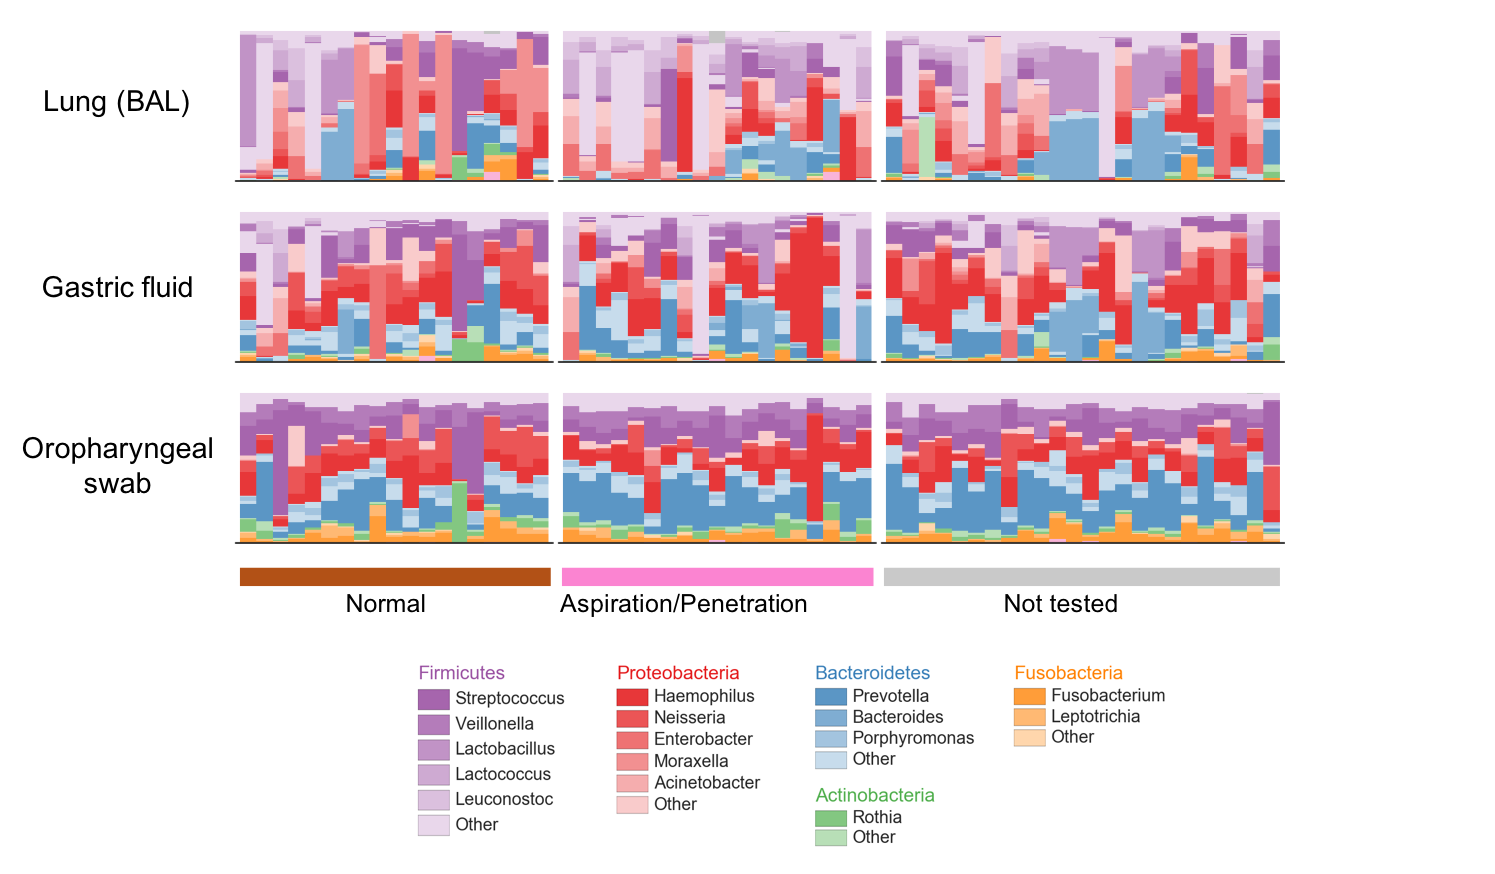
\includegraphics[width=1.2\textwidth]{community_overview_whitebckg.png}
        \caption{\textbf{Aerodigestive communities have similar predominant genera.} Bar plots showing relative abundances of aerodigestive OTUs collapsed to the genus level. Each column corresponds to one patient who had all three aerodigestive sites sequenced (N $=$ 19 non-aspirators, 23 aspirators, 24 untested). Phyla in legend are those with mean abundance $>$ 0.01 across all patients. Any other phyla are colored gray.}
        \label{fig1}
        \end{center}
\end{figure}

\begin{figure}[h]
        \begin{center}
        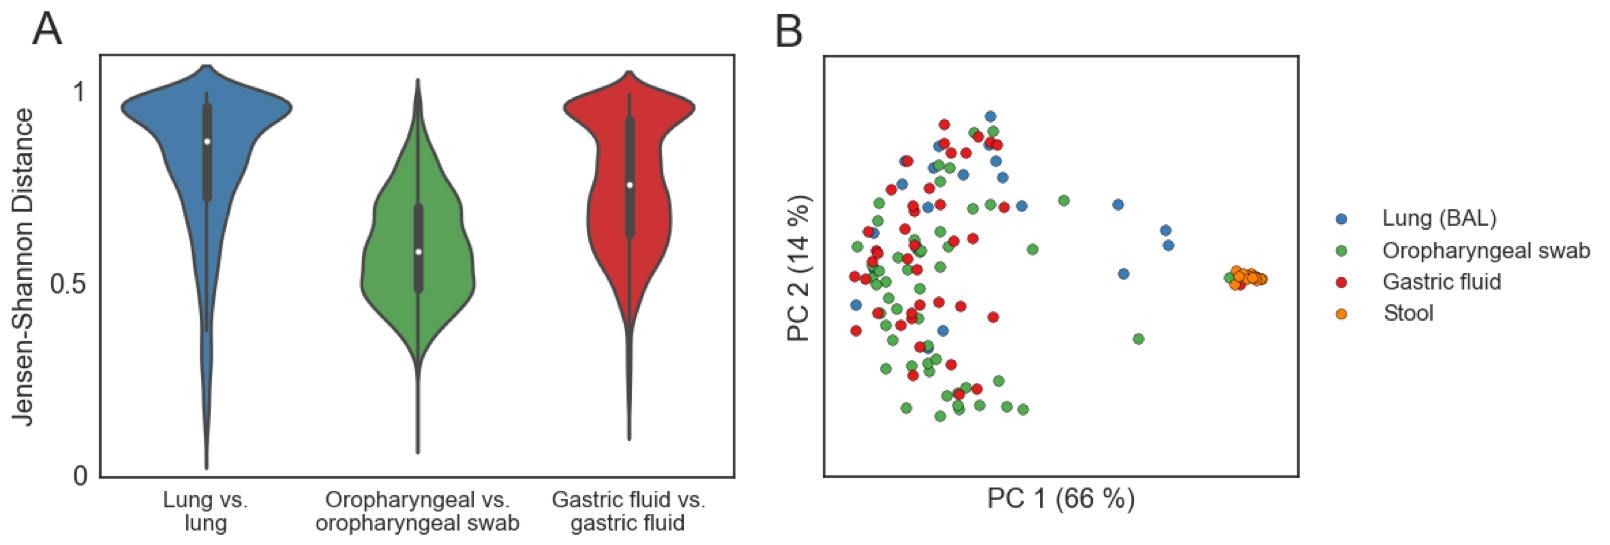
\includegraphics[width=\textwidth]{baseline_aerodigestive_across_patients_whitebckg.png}
        \caption{\textbf{Lung and gastric communities are more variable across people than oropharyngeal communities.} (A) Violin plot of the Jensen-Shannon distance (JSD) between samples from the same site across different patients. A JSD close to 1 indicates that communities are very different (less similar). (B) PCoA plots of aerodigestive and stool microbial communities for all patients in the 2016 sequencing batch (N $=$ 21 BAL, 52 oropharyngeal swab, 43 gastric fluid, and 14 stool samples).}
        \label{fig2}
        \end{center}
\end{figure}

\begin{figure}[h]
        \begin{center}
        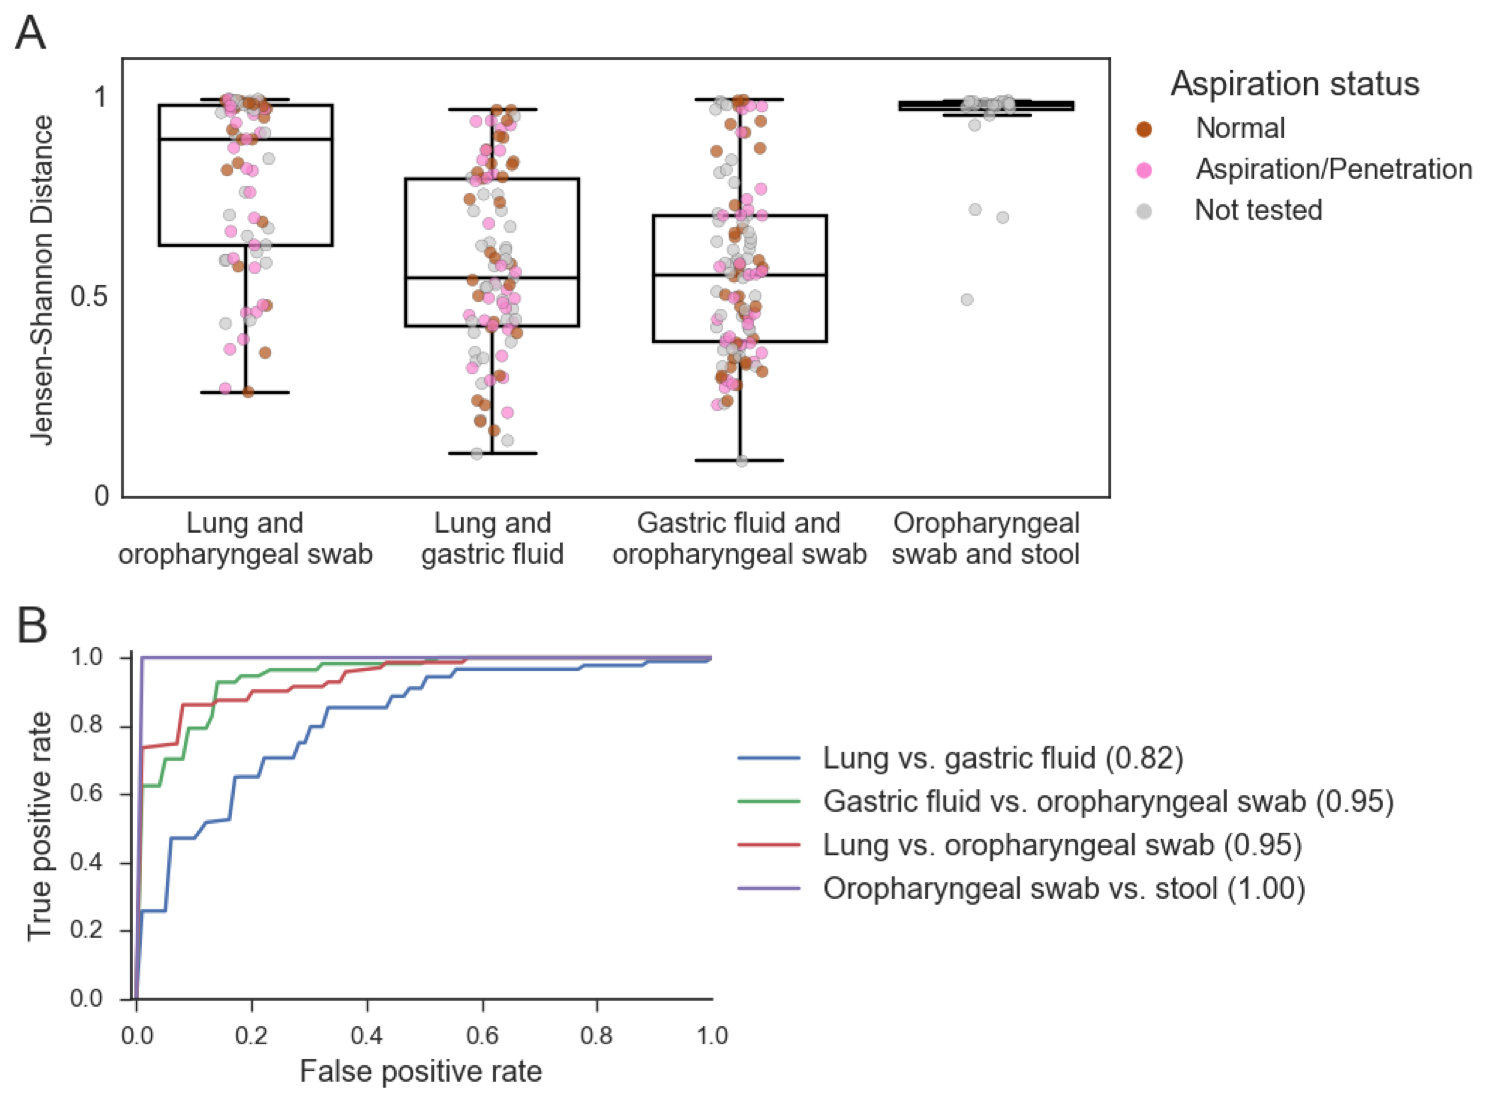
\includegraphics[width=\textwidth]{baseline_aerodigestive_within_patients_whitebckg.png}
        \caption{\textbf{Within patients, aerodigestive communities are similar but lung and oropharynx remain most distinct.} (A) Jensen-Shannon distances between samples from different sites from the same patient. Comparisons between stool and oropharynx are included to contextualize these results, as these are expected to be very different. All comparisons are significant (Wilcoxon rank sums test calculated with Python's \texttt{scipy.stats.ranksums} function) except the lung and gastric fluid vs. gastric fluid and oropharyngeal swab beta diversities (p $=$ 0.6). Lung and oropharyngeal vs. oropharyngeal and stool, p $=$ 0.005. All other comparisons:  $p < 1 \times 10^{-8}$. (B) ROC curve of classifiers distinguishing different aerodigestive sites. Mean areas under the ROC curve (AUCs) are reported in parentheses in the legend.}
        \label{fig3}
        \end{center}
\end{figure}

\begin{figure}[h]
        \begin{center}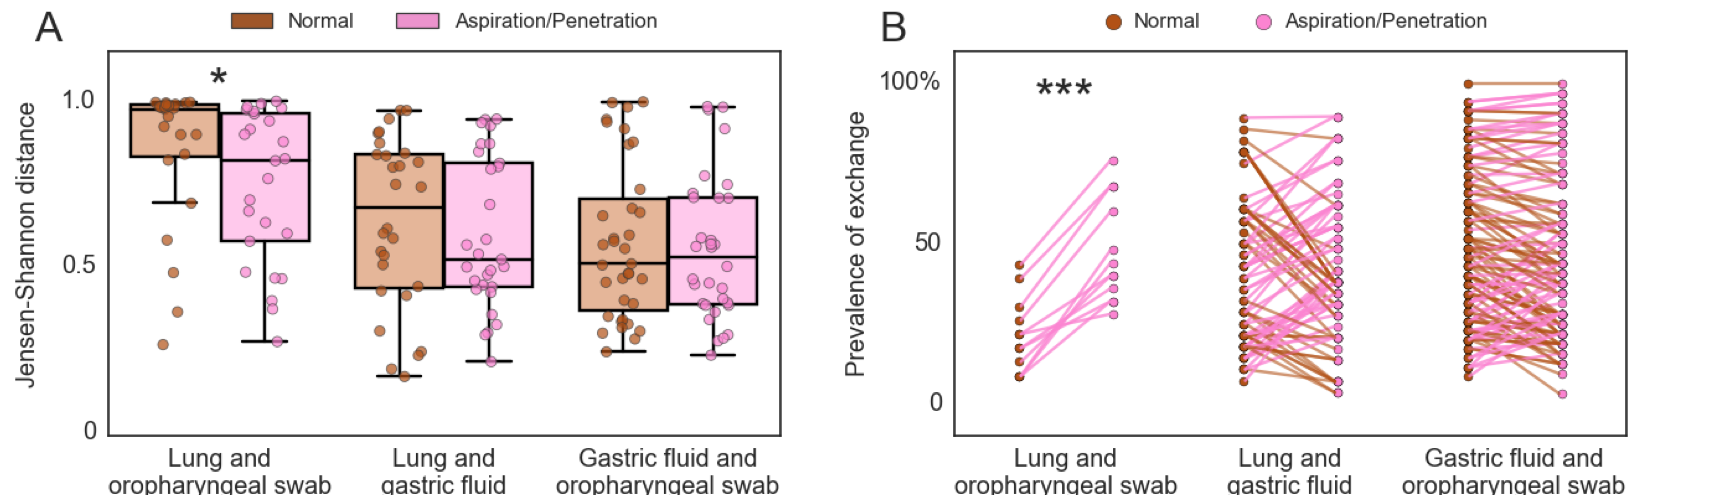
\includegraphics[width=\textwidth]{aspiration_jsd_exchange_whitebckg.png}
        \caption{\textbf{Dysphagia increases aspiration of microbes from the oropharynx but not the stomach} (A) Intra-patient Jensen Shannon distance for different aerodigestive site comparisons in non-aspirators (brown) and aspirators (pink). Each point represents one patient. P-values (Wilcoxon rank sums test, calculated with Python's \texttt{scipy.stats.ranksums} function): lung and oropharyngeal swab $p = 0.04$, lung and gastric fluid $p = 0.5$, gastric fluid and oropharyngeal swab $p = 0.8$. (B) Percentage of patients with the previously defined exchanged microbes present in both of the respective sites (x-axis) in non-aspirators (brown) and aspirators (pink). Each pair of points represents one exchanged OTU. P-values (paired t-test on $log_{10}$ prevalence values, calculated with Python's \texttt{scipy.stats.ttest\_rel} function: lung and oropharyngeal swab $p = 3 \times 10^{-5}$, lung and gastric fluid $p = 0.8$, gastric fluid and oropharyngeal swab $p = 0.09$.}
        \label{fig4}
        \end{center}
\end{figure}

\begin{figure}[h]
        \begin{center}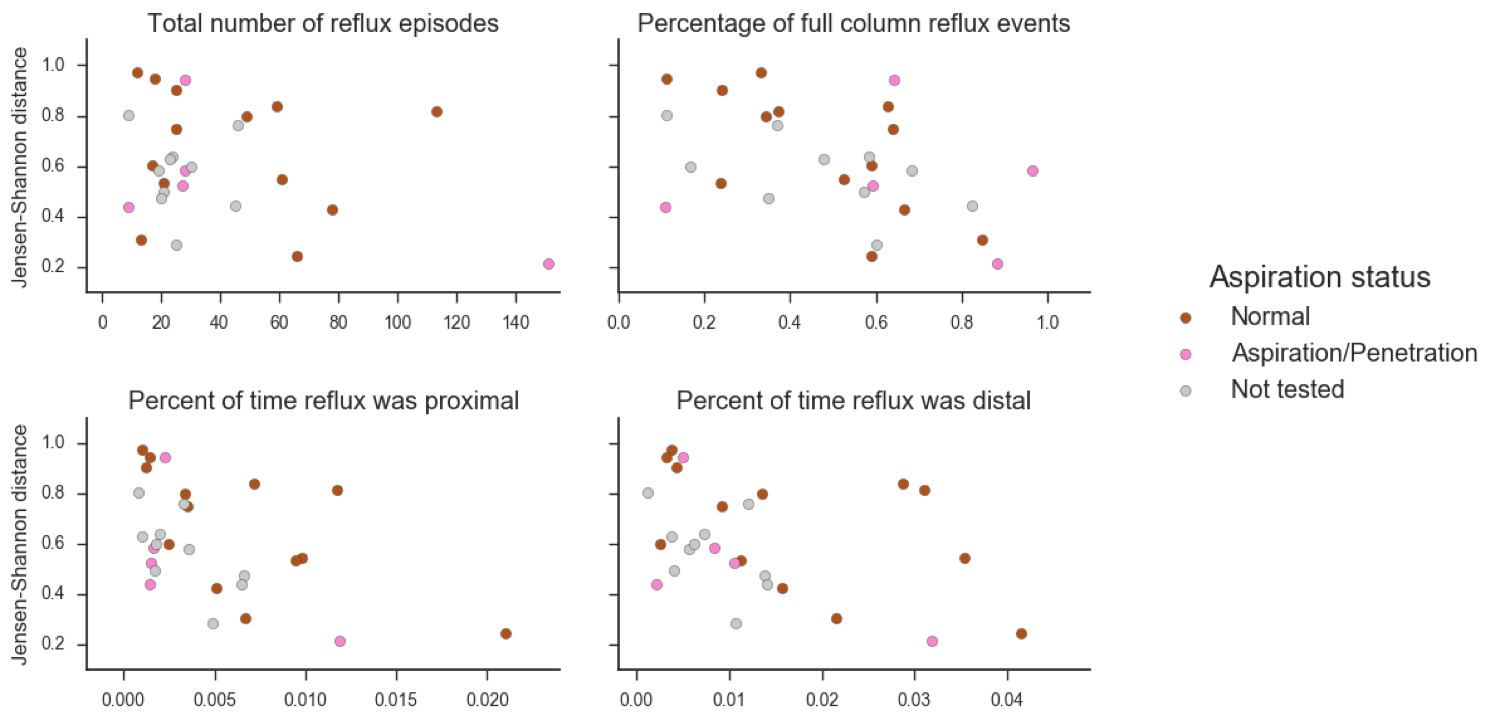
\includegraphics[width=\textwidth]{reflux_correlation_with_bal_gastric.png}
        \caption{\textbf{Reflux severity may correlate with the similarity between lung and gastric communities.} Each plot shows the correlation between different reflux measures and the within-patient Jensen-Shannon distance between BAL and gastric fluid samples. Points are colored according to aspiration status. All reflux measures include both acid- and non-acid reflux. Spearman correlation and p-values: total number of reflux episodes $\rho_s = -0.14, p = 0.5$, percentage of full column reflux events $\rho_s = -0.41, p = 0.03$, percent of time reflux was proximal $\rho_s = -0.47, p = 0.01$, percent of time reflux was distal $\rho_s = -0.43, p = 0.02$.}
        \label{fig5}
        \end{center}
\end{figure}

\FloatBarrier
\newpage

\begin{singlespace}
\bibliographystyle{unsrtnat}
\bibliography{aspiration/aspiration_refs.bib}
\end{singlespace}
